%%%%%%%%%%%%%%%%% DO NOT CHANGE HERE %%%%%%%%%%%%%%%%%%%% {
    \documentclass[12pt,letterpaper]{article}
    \usepackage{fullpage}
    \usepackage[top=2cm, bottom=4.5cm, left=2.5cm, right=2.5cm]{geometry}
    \usepackage{amsmath,amsthm,amsfonts,amssymb,amscd}
    \usepackage{lastpage}
    \usepackage{enumerate}
    \usepackage{fancyhdr}
    \usepackage{mathrsfs}
    \usepackage{xcolor}
    \usepackage{graphicx}
    \usepackage{listings}
    \usepackage{hyperref}
    \usepackage{float} 
    \usepackage{subfigure}
    \definecolor{codegreen}{rgb}{0,0.6,0}
    \definecolor{codegray}{rgb}{0.5,0.5,0.5}
    \definecolor{codepurple}{rgb}{0.58,0,0.82}
    \definecolor{backcolour}{rgb}{0.95,0.95,0.92}
    
    \lstdefinestyle{mystyle}{
        backgroundcolor=\color{backcolour},   
        commentstyle=\color{codegreen},
        keywordstyle=\color{magenta},
        numberstyle=\tiny\color{codegray},
        stringstyle=\color{codepurple},
        basicstyle=\ttfamily\footnotesize,
        breakatwhitespace=false,         
        breaklines=true,                 
        captionpos=b,                    
        keepspaces=true,                 
        numbers=left,                    
        numbersep=5pt,                  
        showspaces=false,                
        showstringspaces=false,
        showtabs=false,                  
        tabsize=2
    }

    \hypersetup{%
      colorlinks=true,
      linkcolor=blue,
      linkbordercolor={0 0 1}
    }
    
    \setlength{\parindent}{0.0in}
    \setlength{\parskip}{0.05in}
    %%%%%%%%%%%%%%%%%%%%%%%%%%%%%%%%%%%%%%%%%%%%%%%%%%%%%%%%%% }
    
    %%%%%%%%%%%%%%%%%%%%%%%% CHANGE HERE %%%%%%%%%%%%%%%%%%%% {
    \newcommand\course{ECE 271A}
    \newcommand\semester{Fall 2019}
    \newcommand\hwnumber{\#2}                 % <-- ASSIGNMENT #
    \newcommand\NetIDa{Jiaming Lai}           % <-- YOUR NAME
    \newcommand\NetIDb{A53314574}           % <-- STUDENT ID #
    %%%%%%%%%%%%%%%%%%%%%%%%%%%%%%%%%%%%%%%%%%%%%%%%%%%%%%%%%% }
    
    %%%%%%%%%%%%%%%%% DO NOT CHANGE HERE %%%%%%%%%%%%%%%%%%%% {
    \pagestyle{fancyplain}
    \headheight 35pt
    \lhead{\NetIDa}
    \lhead{\NetIDa\\\NetIDb}                 
    \chead{\textbf{\Large Assignment \hwnumber}}
    \rhead{\course \\ \semester}
    \lfoot{}
    \cfoot{}
    \rfoot{\small\thepage}
    \headsep 1.5em
    %%%%%%%%%%%%%%%%%%%%%%%%%%%%%%%%%%%%%%%%%%%%%%%%%%%%%%%%%% }
    
    \begin{document}
     
    \section*{Computer Problem Solution}
    % If the Problem is divided into items, use "enumerate"
    \begin{enumerate}[a)]
        %%%%%%%%%%%%%%%%%%%%%%%%%%%%%%%%%%%%%%%%%%%%%%%%%%%%%%%%%%
        % Problem (a)
        %%%%%%%%%%%%%%%%%%%%%%%%%%%%%%%%%%%%%%%%%%%%%%%%%%%%%%%%%%
        \item 
        
        \textbf{Solution}:\\
        Using the results of problem 2, the maximum likelihood estimate for the prior probabilities is following:
        \begin{equation}
            P_Y(cheetah) = N_{FG} / (N_{FG} + N_{BG}) = 0.1919 \nonumber
        \end{equation}
        \begin{equation}
            P_Y(grass) = N_{BG} / (N_{FG} + N_{BG}) = 0.8081 \nonumber
        \end{equation}
        where 
        \begin{itemize}
            \item[] $N_{BG}$ is the number of grass samples
            \item[] $N_{FG}$ is the number of cheetah samples
        \end{itemize}
        These estimates are actually the same as the estimates that I obtained in Homework\#1. It implies that the prior probabilities
        could be estimated by using proportion of each states in the samples if we have enough or big number of samples.\\
        \\
        The histogram is shown below. Mark cheetah to 1 and grass to 0. We could use the histogram to estimate $P_Y(cheetah)$ and $P_Y(grass)$. The result is the same as
        ML estimates.
        \begin{figure}[H]
            \centering 
            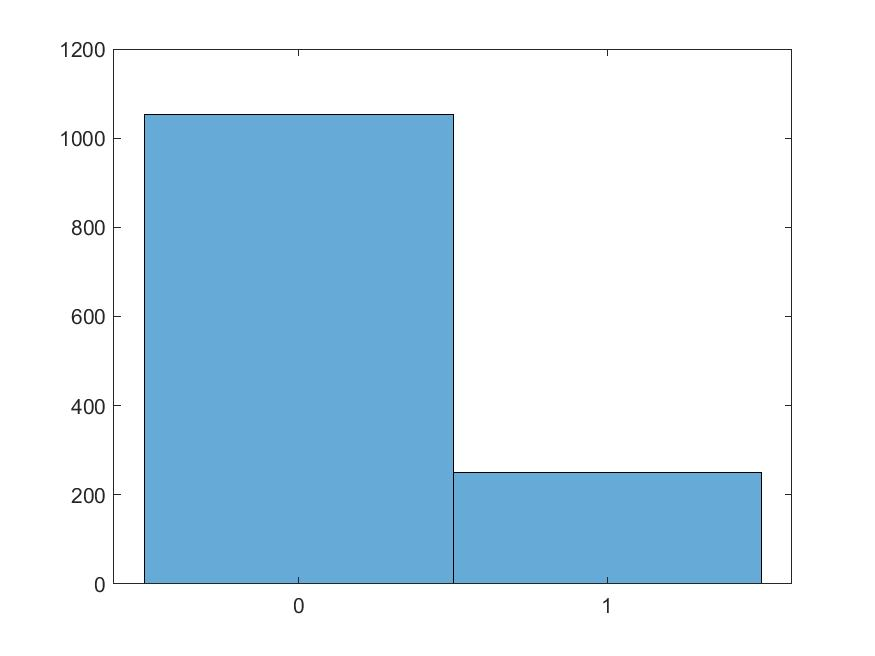
\includegraphics[width=0.45\textwidth]{Images/histogram.jpg}
            \label{Fig.histogram}
        \end{figure}

        %%%%%%%%%%%%%%%%%%%%%%%%%%%%%%%%%%%%%%%%%%%%%%%%%%%%%%%%%%
        % Problem (b)
        %%%%%%%%%%%%%%%%%%%%%%%%%%%%%%%%%%%%%%%%%%%%%%%%%%%%%%%%%%
        \item 
        
        \textbf{Solution}:\\
        The marginal densities for two classes
        \begin{equation}
            P_{x_k|Y}(x_k|cheetah)\ and\ P_{x_k|Y}(x_k|grass),\ k=1,2,\ldots,64 \nonumber
        \end{equation}
        are shown below on Figure 1. The blue line represents $P_{x_k|Y}(x_k|cheetah)$ and the red line
        represents $P_{x_k|Y}(x_k|grass)$.
        \begin{figure}[H]
            \centering 
            \subfigure{
            \label{Fig.sub.1}
            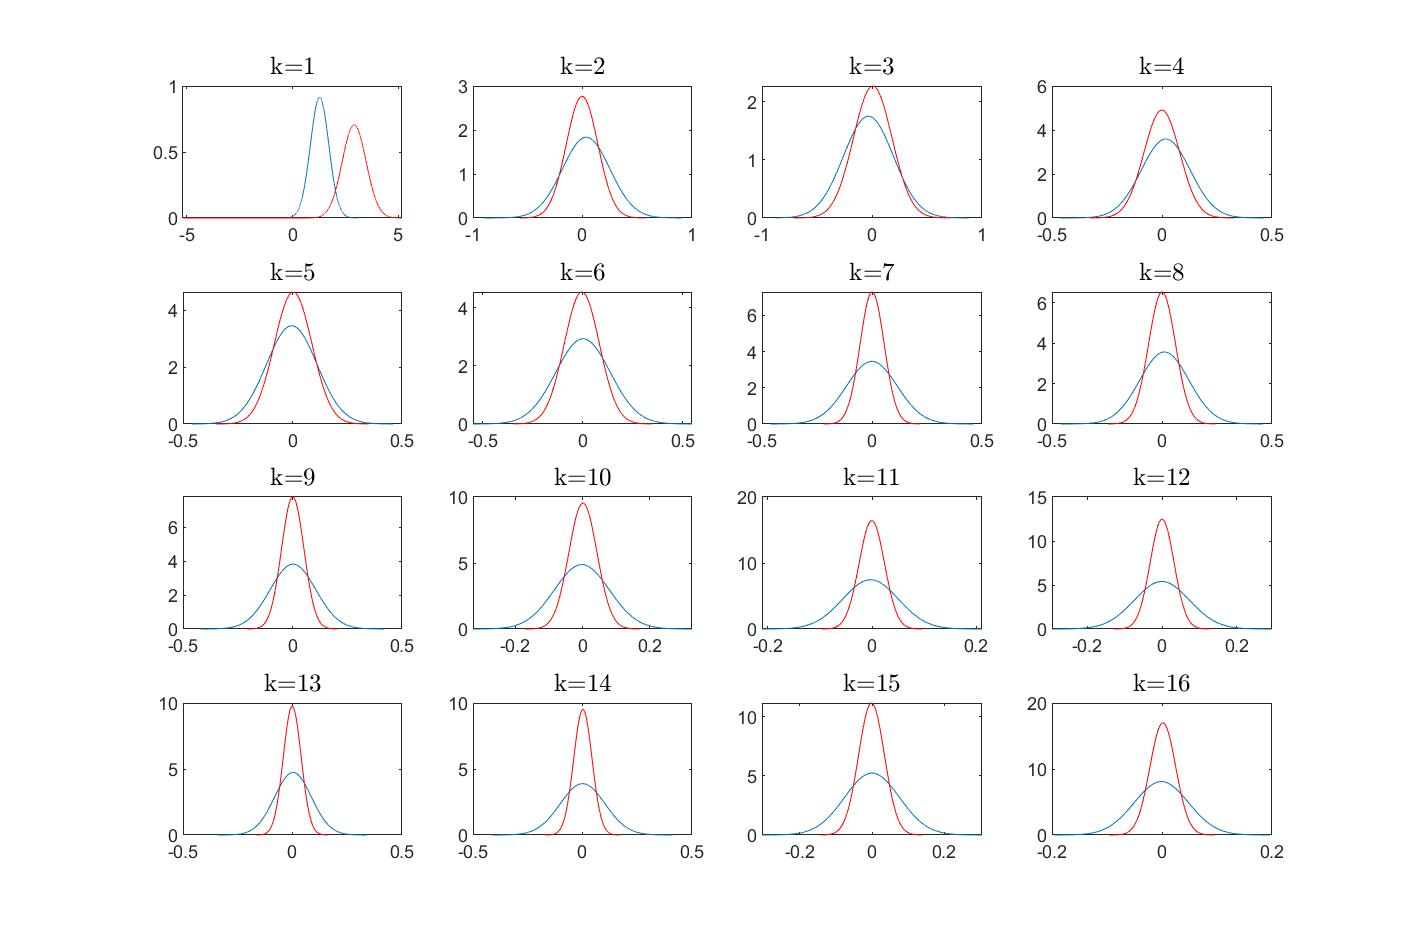
\includegraphics[width=0.45\textwidth]{Images/subplot1.jpg}}
            \subfigure{
            \label{Fig.sub.2}
            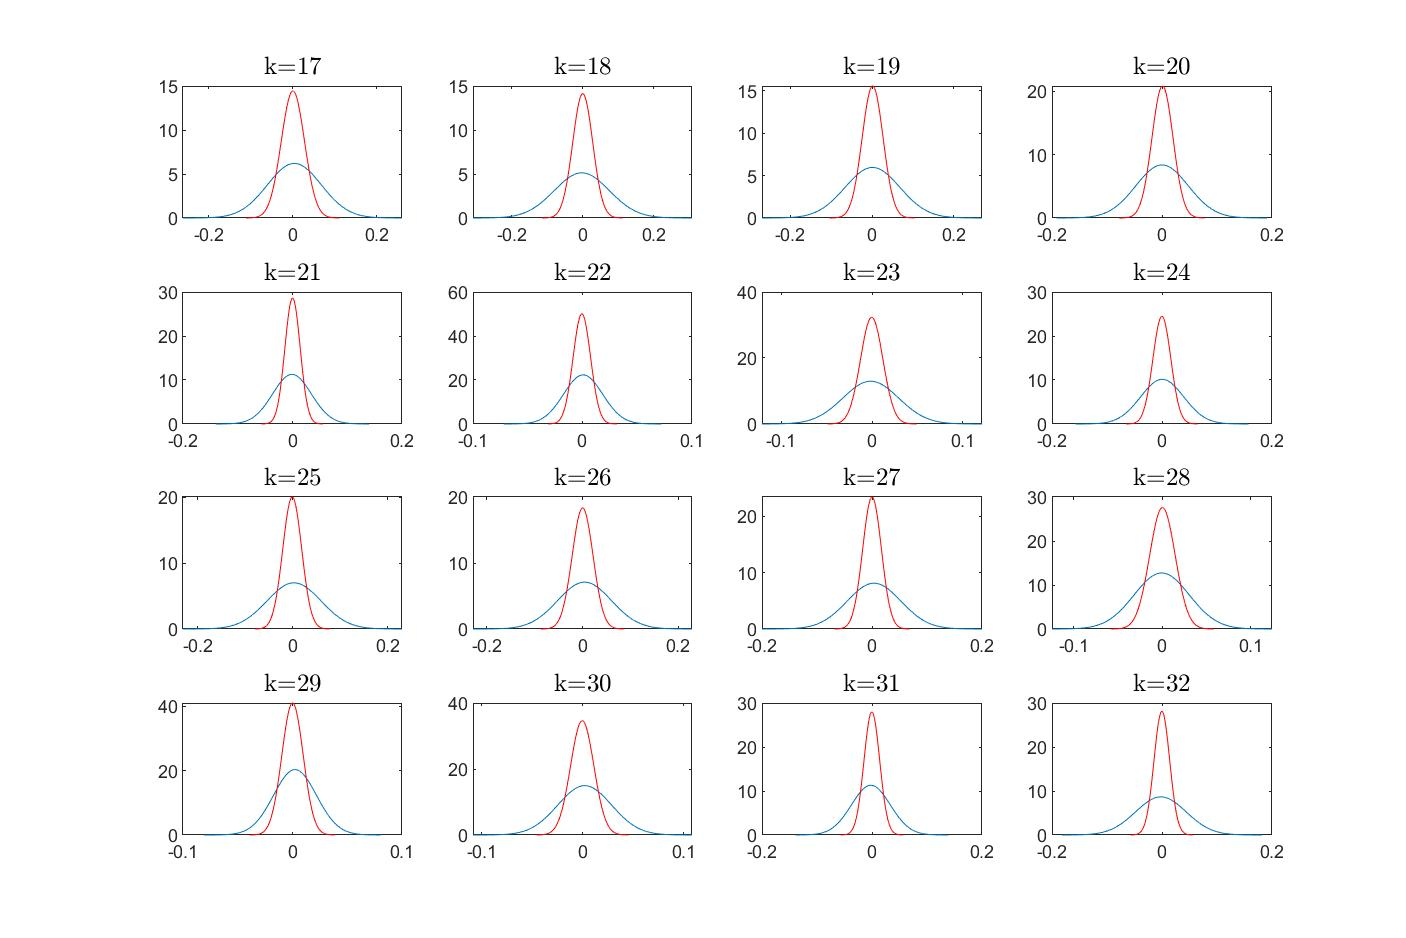
\includegraphics[width=0.45\textwidth]{Images/subplot2.jpg}}
            \label{Fig.main}
        \end{figure}
        \begin{figure}[H]
            \centering 
            \subfigure{
            \label{Fig.sub.3}
            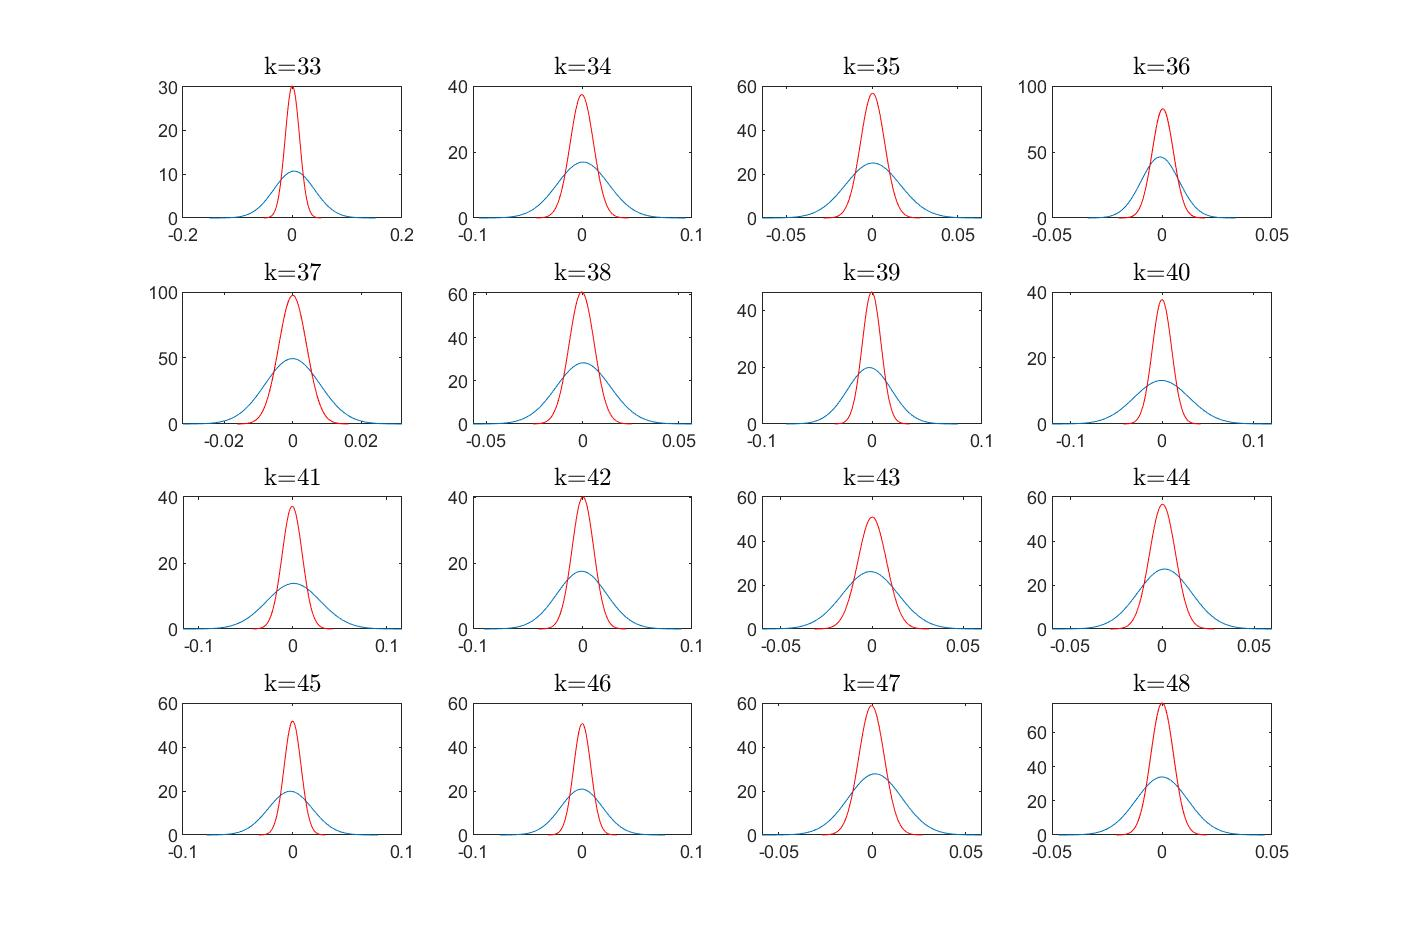
\includegraphics[width=0.45\textwidth]{Images/subplot3.jpg}}
            \subfigure{
            \label{Fig.sub.4}
            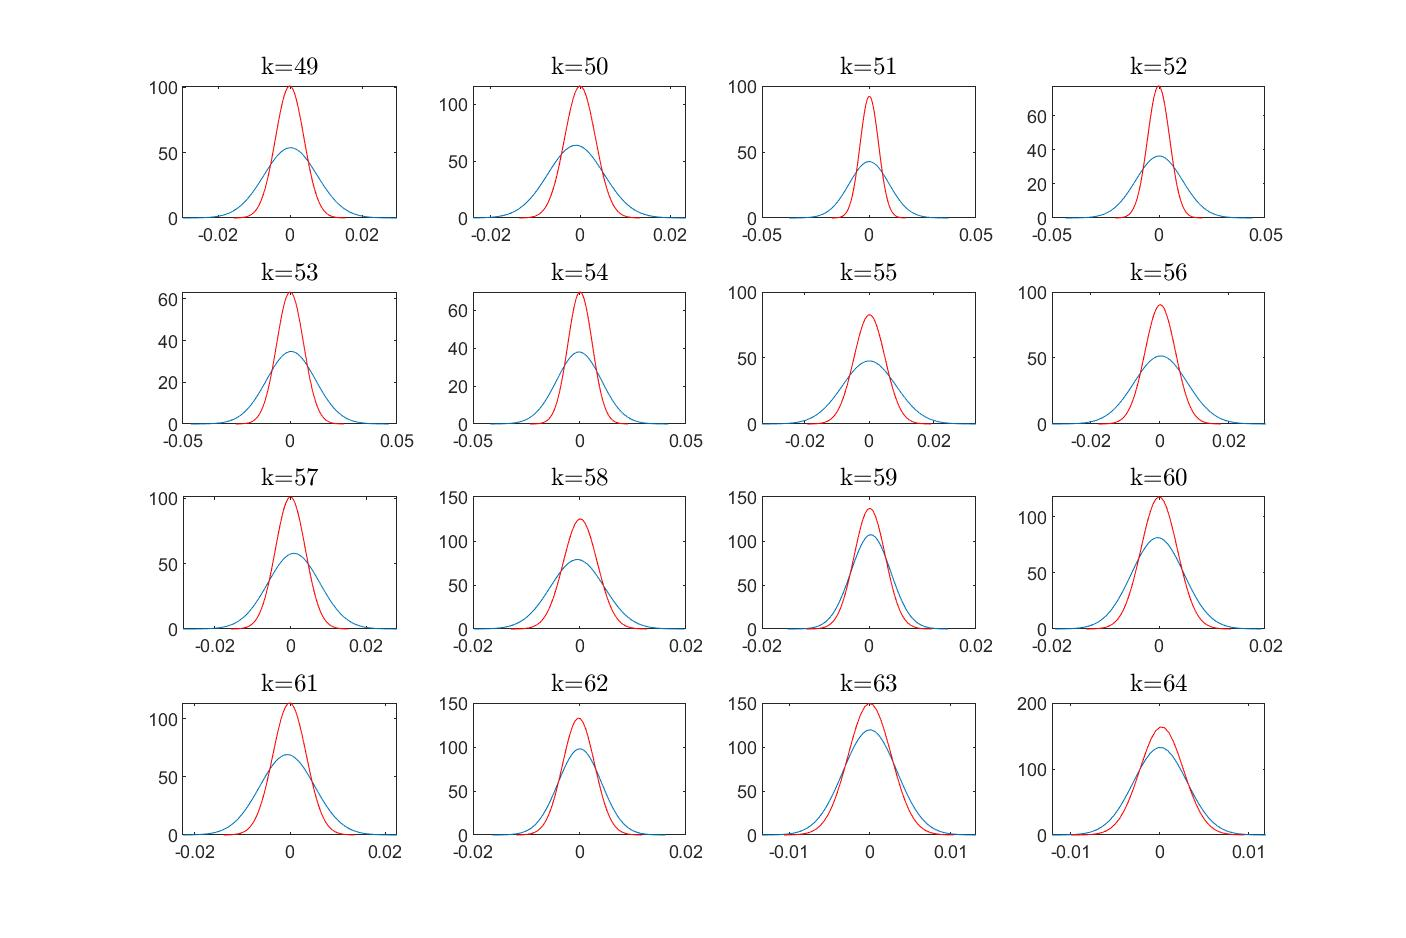
\includegraphics[width=0.45\textwidth]{Images/subplot4.jpg}}
            \caption{Marginal densities for two classes}
            \label{Fig.main}
        \end{figure}
        By visual inspection, the best 8 features and worst 8 features are:
        \begin{itemize}
            \item[] best 8 features:[1,18,25,27,32,33,40,41]
            \item[] worst 8 features:[3,4,5,59,60,62,63,64]
        \end{itemize}
        The plots of the marginal densities for the best-8 and worst-8 features are shown below:
        \begin{figure}[H]
            \centering 
            \subfigure[Best 8 features]{
            \label{Fig.sub.1}
            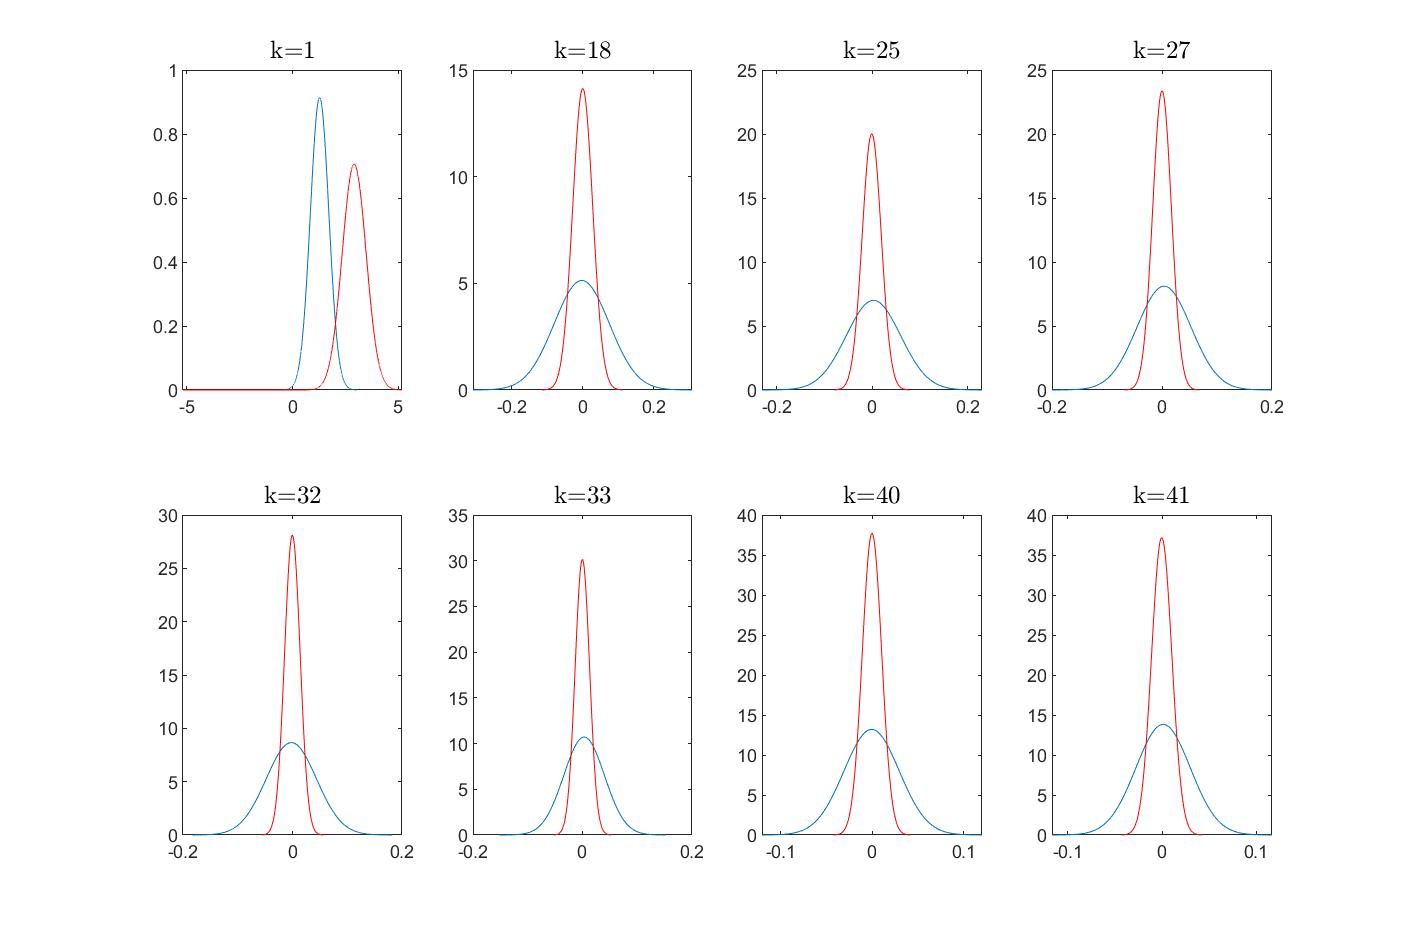
\includegraphics[width=0.8\textwidth]{Images/subplot_best8features.jpg}}
        \end{figure}
        \begin{figure}[H]
            \centering 
            \subfigure[Worst 8 features]{
            \label{Fig.sub.2}
            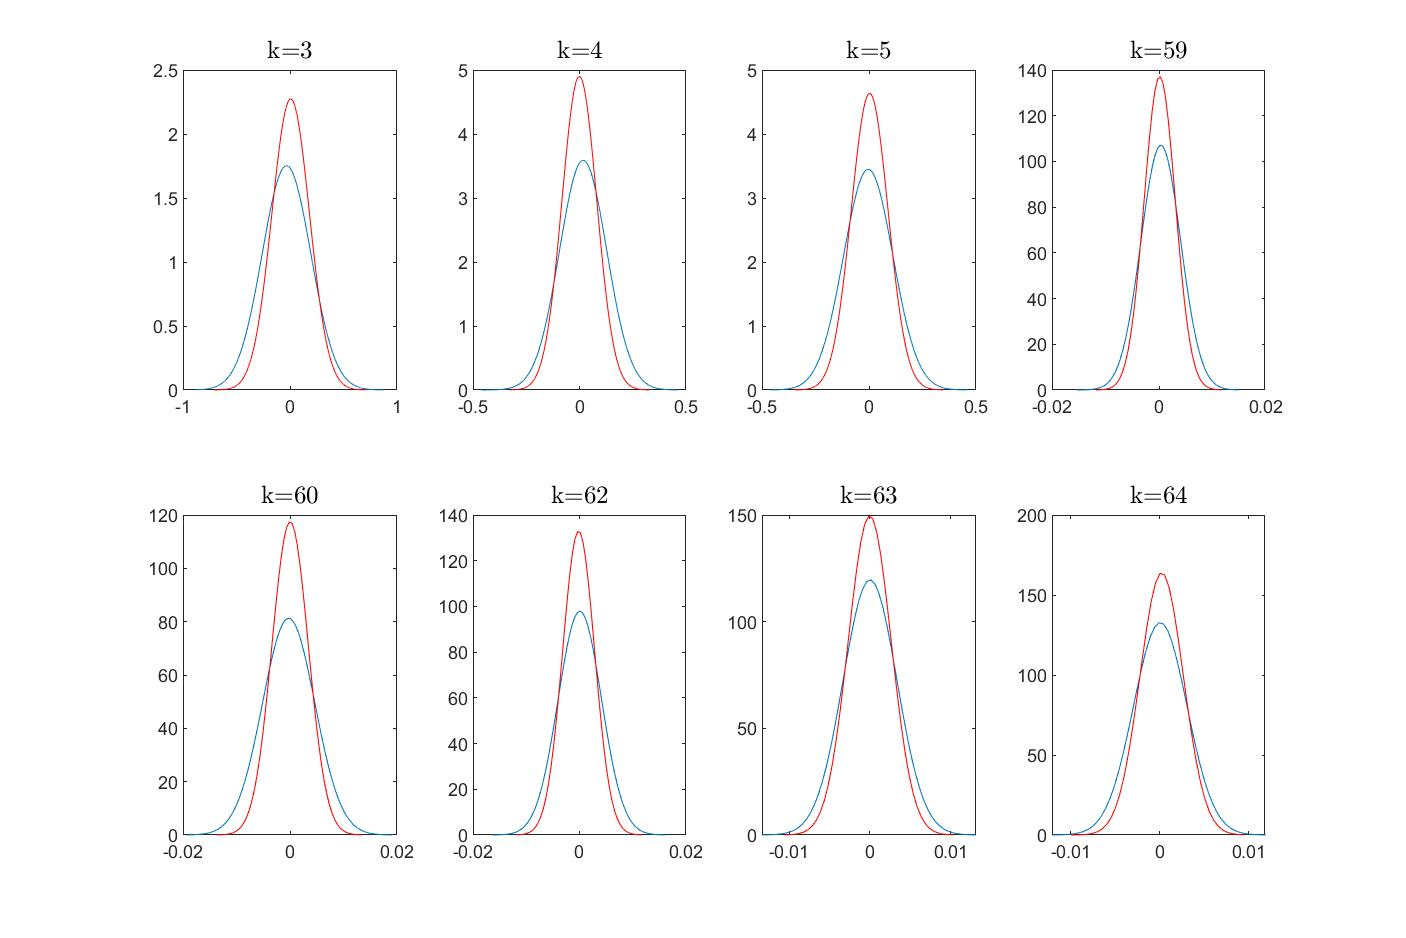
\includegraphics[width=0.8\textwidth]{Images/subplot_worst8features.jpg}}
            \caption{Marginal densities for the best-8 and worst-8 features}
            \label{Fig.bestandworst}
        \end{figure}

        %%%%%%%%%%%%%%%%%%%%%%%%%%%%%%%%%%%%%%%%%%%%%%%%%%%%%%%%%%
        % Problem (c)
        %%%%%%%%%%%%%%%%%%%%%%%%%%%%%%%%%%%%%%%%%%%%%%%%%%%%%%%%%%
        \item  
        \textbf{Solution}:\\
        By using Bayesian decision rule, we can compare the proportion of conditional probabilities of two classes, compare the result with
        the threshold and mask the top left corner of the 8*8 block as 1, regarding this pixel belongs to cheetah. Otherwise, we mask 0.
        \begin{equation}
            \frac{P_{X|Y}(x|cheetah)}{P_{X|Y}(x|grass)} > T = \frac{P_Y(grass)}{P_Y(cheetah)} \nonumber
        \end{equation}
        where 
        \begin{itemize}
            \item[] $P_{X|Y}(x|cheetah)$ and $P_{X|Y}(x|grass)$ are conditional probabilities of two classes.
            \item[] $P_Y(cheetah)$ and $P_Y(grass)$ are the ML estimates we get from training data.
            \item[] $T$ is the threshold.
        \end{itemize}
        $P_{X|Y}(x|cheetah)$ and $P_{X|Y}(x|grass)$ is calculated using the following equation
        \begin{equation}
            P_{X|Y}(x|i)= \frac{1}{\sqrt{(2\pi)^d|\Sigma_i|}}exp\{-\frac{1}{2}(x-\mu_i)^T\Sigma_i^{-1}(x-\mu_i)\} \nonumber
        \end{equation}
        The classification results using 64-dimensional Gaussians and 8-dimensional Gaussians associated with the best 8 features
        are shown below. Compare it with the ground truth provided in image \textbf{cheetah mask.bmp} and compute the probability of error.
        The probability of error is also shown in the figure below.
        \begin{figure}[H]
            \centering 
            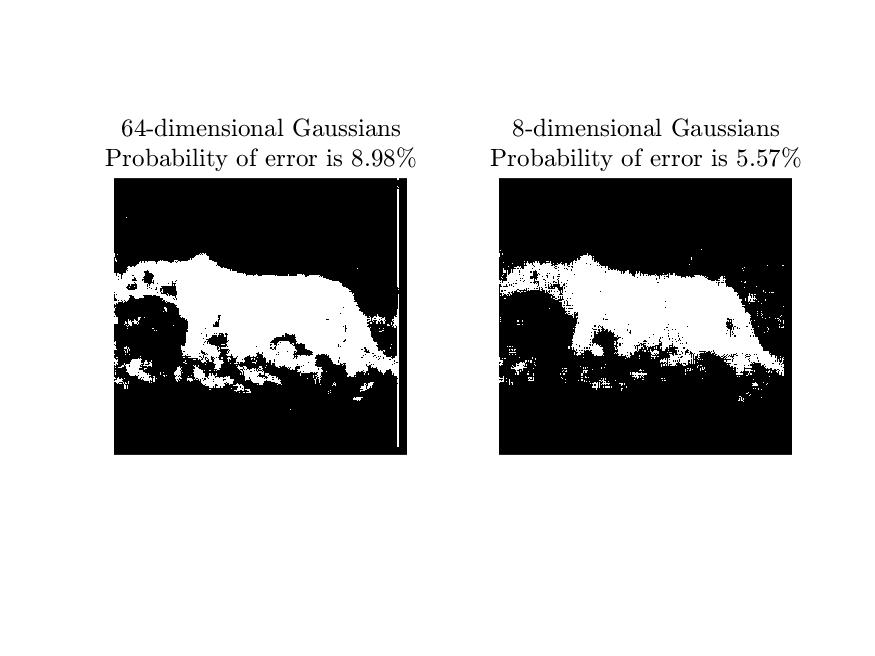
\includegraphics[width=0.8\textwidth]{Images/segmentation.jpg}
            \caption{Classification results}
            \label{Fig.main}
        \end{figure}
        Obviously, the classification performance of 8-dimensional Gaussians associated with the best 8 features is better than the 64-dimensional
        Gaussians. My explanation is that while we add more features to the best 8 features, the probability density distribution of
        $P_{X|Y}(x|cheetah)$ and $P_{X|Y}(x|grass)$ will get closer, bacause some features' marginal densities are very similiar, just like the worst
        8 features we shown above. Thus, it makes Bayesian decision rule based classification perform worse. 
    \end{enumerate}

    \section*{Appendix}
    The following is the Matlab code.

    \subsection{HW2\_solution.m}
    \lstset{style=mystyle}
    \lstinputlisting[language=Octave]{HW2_solution.m}

    \subsection{fun\_mean.m}
    The function for calculating ML mean.
    \lstset{style=mystyle}
    \lstinputlisting[language=Octave]{fun_mean.m}

    \subsection{fun\_cov.m}
    The function for calculating covariance matrix and ML variance.
    \lstset{style=mystyle}
    \lstinputlisting[language=Octave]{fun_cov.m}

    \subsection{fun\_gaussian.m}
    \lstset{style=mystyle}
    \lstinputlisting[language=Octave]{fun_gaussian.m}

    \subsection{fun\_mvgaussian.m}
    \lstset{style=mystyle}
    \lstinputlisting[language=Octave]{fun_mvgaussian.m}

    \end{document}